%%%%%%template by Daniel Parker
%%%%%%http://dug.math.brown.edu/
\documentclass[10pt,twoside]{article}
%%%%%%%%%packages%%%%%%%%%
\usepackage{amsmath}
\usepackage{amssymb}
\usepackage{amsfonts}
\usepackage{amsthm}
\usepackage{mathrsfs}
\usepackage{mathtools}
\usepackage{colonequals} 	
\usepackage{graphicx}
\usepackage{fancyhdr}
\usepackage{multirow}
\usepackage{siunitx}
\usepackage{tikz}
\usepackage[headings]{fullpage}

%%%%%%%%%header%%%%%%%%%
\pagestyle{fancy}
\fancyhead{} % clear all header fields
\renewcommand{\headrulewidth}{0.2pt}
\fancyhead[RO,LE]{\bfseries \hspace{1in}\rightOne\phantom{\hspace{1in}}\\ \hspace{1in}\rightTwo\hspace{1in}}
\fancyhead[RE,LO]{\bfseries \hspace{1in}\leftOne\phantom{\hspace{1in}}\\ \hspace{1in}\leftTwo\hspace{1in}}
\fancyhead[C]{\bfseries \centerOne\\\centerTwo}
\fancyfoot{}
\setlength{\voffset}{-1in+1.5em}
\fancyheadoffset{1in}
\addtolength{\textheight}{1in}

%%%%%%%%%theorem environment and numbering%%%%%%%%%
%%%%%%%%%uses amsthm package
\newtheorem{thm}{Theorem}
\newtheorem{prop}[thm]{Proposition}
\newtheorem{lm}[thm]{Lemma}
\newtheorem{defn}[thm]{Definition}
\newtheorem{rem}[thm]{Remark}
\newtheorem{cl}{Claim}[thm]
\newtheorem{cor}[thm]{Corollary}

\theoremstyle{definition}
\newtheorem{eg}[thm]{Example}

%%%%%%%%%exercise numbering%%%%%%%%%
\newtheoremstyle{exercise}{}{}{\itshape}{}{\bfseries}{:}{.5em}{\thmname{#1} \thmnumber{#2}\thmnote{(#3)}}
\theoremstyle{exercise}
\newtheorem{ex}{Exercise}
\newcommand{\nextex}[1]{\begin{ex}\end{ex}}
\newcommand{\nextexP}[1]{\begin{ex}#1\end{ex}}
\newcommand{\setex}[1]{\setcounter{ex}{#1-1}\begin{ex}\end{ex}}
\newcommand{\setexP}[2]{\setcounter{ex}{#1-1}\begin{ex}#2\end{ex}}

%%%%%%%%%notation shortcuts%%%%%%%%%
\newcommand{\R}{\mathbb{R}}
\newcommand{\Q}{\mathbb{Q}}
\newcommand{\Z}{\mathbb{Z}}
\newcommand{\N}{\mathbb{N}}
\newcommand{\F}{\mathbb{F}}
\newcommand{\C}{\mathbb{C}}


\newcommand{\n}[1]{\left| #1 \right|}%%adjustable-height norm shortcut
\newcommand{\set}[2]{\left\{#1\left|\; #2 \right. \right\}}%%set notation shortcut with a line
\newcommand{\setc}[2]{\left\{#1\; :\; #2 \right\}}%%set notation shortcut with a colon
\newcommand{\st}[1]{\left\{#1\right\}}%%set notation shortcut with no condition
\newcommand{\ce}{\colonequals}%%shortcut to write \colonequals

\newcommand{\bvi}{\hat{\mathbf{i}}} %basis vector i
\newcommand{\bvj}{\hat{\mathbf{j}}} %basis vector j
\newcommand{\bvk}{\hat{\mathbf{k}}} %basis vector k
\newcommand{\bvr}{\hat{\mathbf{r}}} %basis vector r
\newcommand{\bvt}{\hat{\mathbf{\theta}}}%basis vector theta
\newcommand{\bvx}{\hat{\mathbf{x}}} %basis vector x
\newcommand{\bvy}{\hat{\mathbf{y}}}%basis vector y
\renewcommand{\v}[1]{\boldsymbol{#1}}%%shortcut to make a vector N.B. this overwrites the default command for \v which makes a caret over the letter

\newcommand{\aut}{\operatorname{Aut}}
\newcommand{\mor}{\operatorname{Mor}}
\newcommand{\chr}{\operatorname{char}}
\newcommand{\spn}{\operatorname{span}}
\newcommand{\tr}{\operatorname{Tr}}
\newcommand{\im}{\operatorname{Im}}

\DeclareMathOperator\arctanh{arctanh}


%%%MODIFY THESE LINES TO CHANGE THE HEADER
\newcommand{\leftOne}{Brown University}
\newcommand{\leftTwo}{Prof. Dell'Antonio}
\newcommand{\centerOne}{Lensing Formalism}
\newcommand{\centerTwo}{14 January  2013}
\newcommand{\rightOne}{\thepage}
\newcommand{\rightTwo}{Dan Parker}

\begin{document}
The following document includes most of the lensing formalism behind the simulations. This should be sufficient to understand the lensing mass distributions included in the simulations, and how the distortions are set up, including units. The first part discusses lensing in general, then specializes to the NFW profile, and finally looks at the unit conversions necessary in performing simulations.

\section{Lensing Formalism}
This discussion is very brief. See e.g. \cite{Narayan:1996ba} or \cite{VanWaerbeke:2003uq} for more information.

In the weak gravitational field limit, gravitational lensing is given by the lens equation \cite{Narayan:1996ba}
\begin{equation}
		\v{\beta}(\v{\theta}) = \v{\theta} - \v{\alpha}(\v{\theta})
		\label{eq:lens}
\end{equation}
where $\v{\beta}$ is the true angular position, $\v{\theta}$ is the observed angular position, and $\v{\alpha}$ is the deflection angle. (See figure.) All three of these are vectors of two components, which correspond to the angles right and up from some arbitrary optical axis. It is assumed that the area of the sky under consideration is small enough that the curvilinear nature of this coordinate system can be neglected; $\v{\alpha}, \v{\beta}$ and $\v{\theta}$ are small angles and are considered to be elements of $\R^2$. Additionally, the distances from the observer to the lens, observer to the source, and lens to the source are given by $D_\ell$, $D_s$ and $D_{\ell s}$ respectively.

\begin{figure}[h]
		\center
		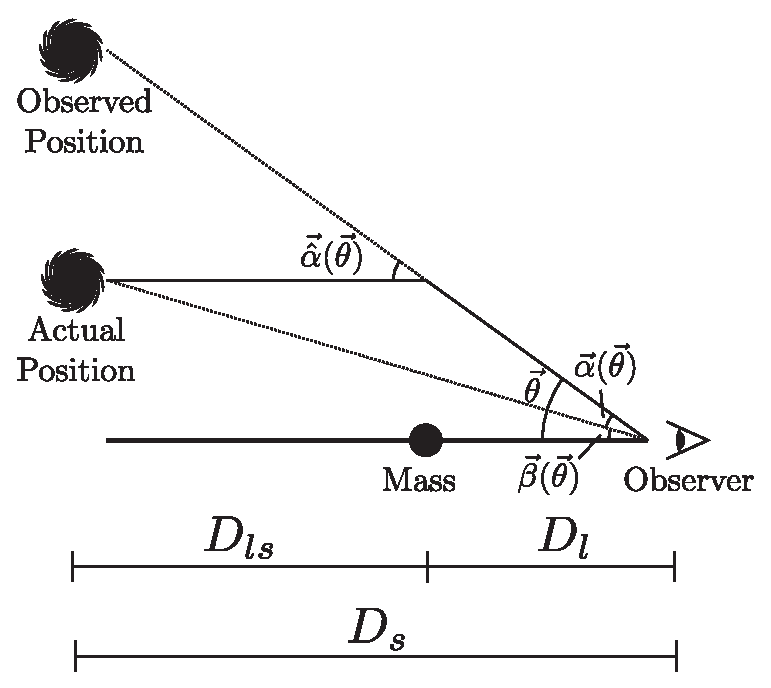
\includegraphics[scale=0.7]{../images/lensing_formalism.eps}
\end{figure}

In the thin lens limit, all the mass is in a single plane $P$ between the source and observer. In this limit, we treat the paths of photons as straight except for a sharp turn when they pass through $P$. Suppose the mass distribution on $P$ is given by $\Sigma(\v{\xi})$, called the surface mass density, where $\v{\xi}$ is a \emph{vector} (not a 2-component angle) in $P$. This confusing point is the focus of Section \ref{sec:units}. Then $\v{\alpha}$ is given by \cite{Narayan:1996ba}
\begin{equation}
		\hat{\v{\alpha}}(\v{\xi}) = \frac{4G}{C^2} \int_P \frac{\left( \v{\xi} - \v{\xi}' \right)\Sigma(\v{\xi})}{\n{\v{\xi} - \v{\xi}'}} \, dA
		\label{eq:thin_lens_deflection}
\end{equation}
where $C$ is the speed of light,\footnote{To prevent confusion with lowercase $c$'s that appear later, this document will always use $C$ to refer to the speed of light.} $G$ is the gravitational constant, and $\hat{\v{\alpha}}$ is a 2-component angle called the reduced deflection. The hat is added to distinguish it from the case where it is a scalar. From the figure and a small angle approximation, it follows that the deflection and reduced deflection are related by
\begin{equation}
		\v{\alpha} = \frac{D_\text{ls}}{D_\text{s}} \hat{\v{\alpha}}
		\label{eq:reduced_deflection}
\end{equation}
Similarly, $\v{\xi} = D_\text{s} \v{\theta}$.

Often, the mass distribution will not actually be planar, but will be concenrated near the plane $P$. More precisely, let $z$ be a coordinate along the path of the light. Then the mass distribution is given by $\rho(\v{\xi}, z)$ where $\rho = 0$ for $\n{z} \ge \varepsilon$ where $\varepsilon$ is some distance which is small compared to the distance between the mass and lightsource or the observer. This is a good approximation in almost all astronomical situations. In this case, $\Sigma$ is given by integrating $\rho$ over the light of sight:
\begin{equation}
		\Sigma(\v{\xi}) \equiv \int_{-\infty}^\infty \rho(\v{\xi}, z), \, dz.
		\label{eq:LOS_approx}
\end{equation}

In the case where $\Sigma$ is radially symmetric, Equation \eqref{eq:thin_lens_deflection} is simplified greatly. Using polar coordinates and applying Gauss's law, the deflection becomes
\begin{equation}
		\hat{\v{\alpha}}(\v{\xi}) =	\hat{\v{\alpha}}(r \hat{\v{r}}) = -\hat{\alpha}(r) \hat{\v{r}}
		\label{eq:radially_symmetric}
\end{equation}
where $r$ is the radial distance from the origin, $\hat{\v{r}}$ is the outward pointing unit normal, and 
\begin{equation}
		\hat{\alpha}(r) = \frac{4G M(r)}{C^2 r}
		\label{eq:radial_deflection}
\end{equation}
with gravitational constant $G$, $C$ the speed of light, and $M(r)$ the mass enclosed up to radius $r$ from the origin \cite{Narayan:1996ba}. More precisely,
\begin{equation}
		M(r) = \int_0^r \int_0^{2\pi} \Sigma(r') \, r' \, d\theta \, dr' = 2\pi \int_0^r r' \Sigma(r') \, dr'.
		\label{eq:mass_enclosed}
\end{equation}

\section{NFW Profile}

One of the most realistic and frequently used mass distributions is the NFW profile. It is spherically symmetric and is a fairly accurate approximation for the mass distribution of astronomical objects, including the associated dark matter, across many scales \cite{Navarro:1995iw}. It has the useful property that most of its properties can be calculated analytically. The profile has several dependent parameters, any two of which are sufficient. The parameters chosen depends on the situation at hand. The best source for information about the NFW paper is \cite{brainerd_wright}.

The NFW profile at redshift $z$ is given by \cite{brainerd_wright}
\begin{equation}
		\rho(r) \equiv \frac{\delta_c \rho_c}{(r/r_s)(1+r/r_s)^2}
		\label{eq:NFW_profile}
\end{equation}
where $\delta_c$, $\rho_c$, and $r_s$ are parameters \cite{brainerd_wright}. The parameters are as follows:
 $\delta_c$ is given by
\begin{equation}
		\delta_c \equiv \frac{200}{3} \frac{c^3}{\ln(1+c) - \frac{c}{1+c}}
		\label{eq:delta_c}
\end{equation}
where $c$ is \emph{NOT} the speed of light, but a dimensionless parameter called the concentration. $\delta_c$ is itself unitless. $\rho_c$ is the critical density for closure of the universe at redshift $z$, and has units of mass per unit volume. It is given by
\begin{equation}
		\rho_c \equiv \frac{3H^2(z)}{8\pi G}
		\label{eq:rho_c}
\end{equation}
where $H(z)$ is the Hubble constant at redshift $z$. Finally, $r_s$ is a characteristic radius for the profile, with units of length, given by
\begin{equation}
		r_s \equiv \frac{r_{200}}{c}
		\label{eq:r_s}
\end{equation}
where $c$ is again the unitless parameter and $r_{200}$ is the virial radius, i.e. the radius such that the enclosed volume has mass density equal to $200 \rho_c$. The mass enclosed by this radius is given by 
\begin{equation}
		M_{200} \equiv M(r_{200}) = \frac{800 \pi}{3} \rho_c r_{200}^3.
		\label{eq:m_200}
\end{equation}

Of course, this profile is given in three spatial dimensions. To be used with the thin lens approximation, we have to compress it along the light of sight. Let $P$ be some plane through the origin and let $z$ be the line through the origin perpedicular to it. Let $R$ be a radial distance on the plane from the origin. Then $\Sigma(R)$, the surface mass density is given by Equation \eqref{eq:LOS_approx}, except with $R$ instead of $\v{\xi}$ because of radial symmetry. To perform the integration, it is necessary to introduce the dimensionless distance variable $x \equiv R/r_s$. This integral is performed in \cite{brainerd_wright}, giving a complicated, but analytic expression.
\begin{equation}
		\Sigma_\text{NFW}(x) = 2r_s \delta_c \rho_c
		\begin{cases}
				\dfrac{1}{x^2-1}\left( 1-\dfrac{2}{\sqrt{1-x^2}} \arctanh \sqrt{\dfrac{1-x}{1+x}}\; \right) & 0 \le x < 1\\[1.2em]
				\dfrac{1}{3} & x=1\\[1.2em]
				\dfrac{1}{x^2-1}\left( 1-\dfrac{2}{\sqrt{x^2-1}} \arctan \sqrt{\dfrac{x-1}{1+x}}\; \right) &  x > 1\\
		\end{cases}
		\label{eq:NFW_surface_mass_density}
\end{equation}
It turns out, however, that this expression is needlessly complicated. By using the complex-valued versions of $\arctan$ or $\arctanh$, either formula holds --- and has the same real value --- for all $x > 0$, with a point discontinuity at $x =1$. Filling this in by continuity, $\Sigma_\text{NFW}$ is actually smooth.

We now want to determine the deflection due to this profile. Since any two parameters are sufficient to describe the profile, $M_{200}$ and $c$ will be used. Equations \eqref{eq:radially_symmetric} and \eqref{eq:radial_deflection} can be used to determine this, but require the enclosed mass to be calculated. Note that the units on $\Sigma_{NFW}$ are mass per unit area. However, $x$ is unitless. This means to find the enclosed mass, $\Sigma_\text{NFW}$ has to be integrated against a dimensionful differential. Since $R = r_sx$, the enclosed mass is
\begin{align}
		M_\text{NFW}(x) \ &=\ 2\pi \int_0^x \Sigma_\text{NFW}(x) R \, dR\\
		\ &=\ 2 \pi r_s^2 \int_0^x \Sigma_\text{NFW}(x') x' \, dx'\\
		\ &=\ 2\pi r_s^2 2 r_s \delta_c \rho_c 
		\int_0^x \, dx' \; x' 
\begin{cases}
		\dfrac{1}{x^{2'}-1}\left( 1-\dfrac{2}{\sqrt{1-x^{2'}}} \arctanh \sqrt{\dfrac{1-x'}{1+x}}\; \right) & 0 \le x' < 1\\[1.2em]
				\dfrac{1}{3} & x'=1\\[1.2em]
				\dfrac{1}{x^{2'}-1}\left( 1-\dfrac{2}{\sqrt{x^{2'}-1}} \arctan \sqrt{\dfrac{x'-1}{1+x'}}\; \right) &  x' > 1\\
		\end{cases}\\[2em]
		\ &=\ 4\pi r_s^3 \delta_c \rho_c
\left[\ln \frac{x}{2} + 
		\begin{cases}
				\frac{2}{\sqrt{1-x^2}} \arctanh \sqrt{\frac{1-x}{1+x}} & 0 \le x < 1\\[1.2em]
				1 & x = 1\\[1.2em]
				\frac{2}{\sqrt{x^2-1}} \arctan \sqrt{\frac{x-1}{1+x}} & x > 1
						\end{cases}
						\right]\\[2em]
\ &=\ 
\frac{M_{200}}{\ln(c+1) - \frac{c}{c+1}}
\left[\ln \frac{x}{2} + 
		\begin{cases}
				\frac{2}{\sqrt{1-x^2}} \arctanh \sqrt{\frac{1-x}{1+x}} & 0 \le x < 1\\[1.2em]
				1 & x = 1\\[1.2em]
				\frac{2}{\sqrt{x^2-1}} \arctan \sqrt{\frac{x-1}{1+x}} & x > 1
						\end{cases}
						\right].
		\label{eq:NFW_enclosed_mass}
\end{align}
The last step comes from applying Equations \eqref{eq:delta_c} - \eqref{eq:m_200} and cancelling. Again, by using $\arctan$ and $\arctanh$ with complex arguments, the first and third piecewise parts give the entire expression, except at $x =1$. Due to the log term, the enclosed mass diverges as $x \to \infty$, albeit quite slowly. Usually the distribution is truncated to account for this. The figure below shows a graph of both $\Sigma_\text{NFW}$ and $M_\text{NFW}$.

\begin{figure}[h]
\center
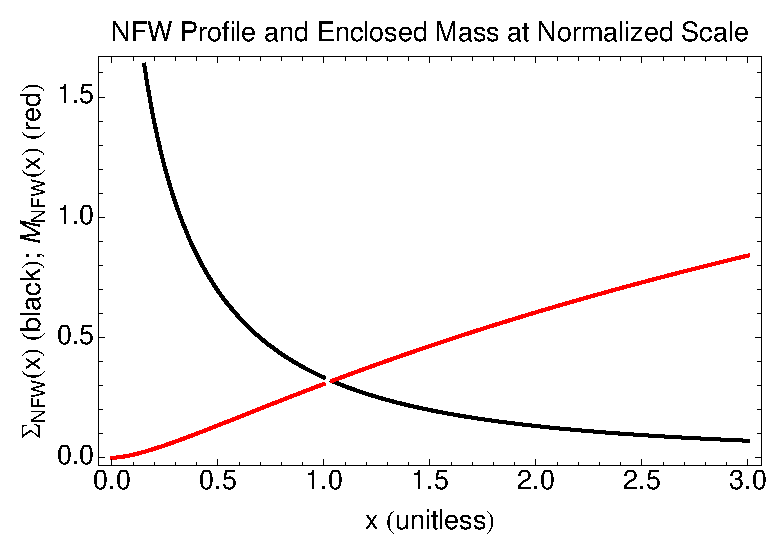
\includegraphics{../images/NFW_Profile.eps}
\end{figure}


\section{Units and Implementation}

\label{sec:units}
In the implementation of the simulations, the task is to calculate $\alpha(r)$ given the mass distribution and it's parameters. This is complicated by the plethora of units involved. Fully six different different units of length or position interact in this calculation:
\begin{enumerate}
		\item Two-component angular position (e.g. $\v{\theta}$, $\v{\beta}$, etc) measured in radians.
		\item Two-component vector position (e.g. $\v{\xi}$).
		\item Angular diameter distance, measured in megaparsecs (e.g. $D_\ell, D_s, D_{\ell s}$).
		\item Dimensionless units used in the equations for the NFW profile (e.g. $x = R/r_s$).
		\item Image pixels, measured in arcseconds.
		\item Sub-pixels used when tabulating the value of $\alpha(r)$ at different radial distances, measured in fractions of a pixel.
\end{enumerate}

Small two-component angles $\v{\theta}$ can be converted to vectors $\v{\xi}$ by
\begin{equation}
		\v{\theta} = D \v{\xi}
		\label{eq:angle_vector_conversion}
\end{equation}
as in elementary geometry. However, $D$ is not a normal length, but is an angular diameter distance, which depends on the cosmology. The angular diameter distance in megaparsecs between two redshifts $z_1$ and $z_2$ is given by
\begin{equation}
		D(z_1,z_2) = \frac{H_0}{z_2+1} \int_{z_1+1}^{z_2+1} \frac{1}{\sqrt{\Omega_M\left( 1+\frac{z}{1+Z_{eq}} \right)z^3 + \Omega_D}} \, dz
		\label{eq:ang_di_dist}
\end{equation}
where $H_0 = 4424.778$ is the Planck constant today, $\Omega_M = 0.315$ and $\Omega_D =0.685$ are respectively the matter and dark energy density of the universe today, and $Z_{eq} = 3391$ is a ratio.

Converting from distances to the dimensionless $x$ distance is given by simply dividing by $r_s$. From \eqref{eq:delta_c} - \eqref{eq:m_200},
\begin{equation}
		r_s = \frac{1}{c}\left( \frac{G M_{200}}{100 H^2(z)} \right)^{1/3y}
		\label{eq:r_s_calculable}
\end{equation}
where as always, $c$ is the parameter and not the speed of light. To actually calculate this, we need to work it out in terms of units. Letting $\tilde{G} = 4.302$ so that $G = \tilde{G} \times 10^3 \frac{\text{pc}}{M_\odot}\left( \frac{km}{s} \right)^2$ and $\tilde{H}_0 = 67.80$ so that $H(z) \approx H(0) = H_0 \frac{km}{s\cdot Mpc}$. Also let $\tilde{M}_{200}$ be the mass parameter value, with $M_{200} = \tilde{M}_{200} \times 10^{14} M_\odot$. Then
\begin{align*}
		r_s(\tilde{M}_{200}, c) \ &=\ \frac{1}{c}\left( \frac{G M_{200}}{100 H^2(z)} \right)^{1/3y}\\
		\ &=\ \frac{1}{c} \left(  \frac{\tilde{G} 10^{-3} \frac{pc}{M_\odot} \tilde{M}_{200} 10^{14} M_\odot}{10^2 \tilde{H}_0^2 \frac{1}{Mpc^2}} \right)^{1/3}\\
		\ &=\ \frac{1}{c} \left( \frac{\tilde{G} 10^{-3} \tilde{M}_{200} pc \times 10^{14}}{10^2 \tilde{H}_0^2 \frac{1}{Mpc^2}} \right)^{1/3}\\
		\ &=\ \frac{1}{c} \left( \frac{\tilde{G} \tilde{M}_{200} \text{Mpc}^3 10^3}{\tilde{H}_0^2} \right)^{1/3}\\
		\ &=\ \frac{10}{c} \left( \frac{\tilde{G} \tilde{M}_{200}}{\tilde{H}_0^2} \right) \text{Mpc}.
\end{align*}
Of course $c$ is the parameter and \emph{not} the speed of light. This is the formula actually used in the program. This can be simplified by using $10 \left( \tilde{G}/\tilde{H}_0^2 \right)^{1/3} = 0.978146$.

In practice, it is better to calculate $\alpha(r)/r$ instead of $\alpha(r)$ because
\begin{equation}
		\v{\alpha}(r) = \begin{bmatrix}
\alpha_x(r)\\
\alpha_y(r)\\
		\end{bmatrix}
		=
 \begin{bmatrix}
		 \alpha(r) \frac{x}{\sqrt{x^2+y^2}}\\
		 \alpha(r) \frac{y}{\sqrt{x^2+y^2}}\\
 \end{bmatrix}
 = 
 \frac{\alpha(r)}{r}
	\begin{bmatrix}
			x\\
			y\\
		  \end{bmatrix}
		\label{eq:alpha_r_components}
\end{equation}

To actually calcuate this in practice, we use the same technique as above. Starting with Equation \eqref{eq:mass_enclosed} and using $\tilde{M}_{200}$ and $\tilde{G}$ as above
\begin{equation}
		\frac{\alpha}{r}(px; \tilde{M}_{200}, c) = \frac{180*3600}{S \pi} \frac{4 \tilde{G}}{9 D_\ell 10^5} M_\text{NFW}\left( \frac{D_\ell}{r_s(\tilde{M}_{200},c)}\frac{\pi}{180} \frac{S}{3600} px \right) \left(  \frac{\pi}{180} \frac{S}{3600} px^2 \right)^{-1} 
		\label{eq:alpha_as_calculated}
\end{equation}
where $S$ is the resolution in arcseconds per pixel ($S=0.03$ for Hubble and $S=0.5$ for LSST), $M_\text{NFW}$ is from Equation \eqref{eq:NFW_enclosed_mass} and $c$, of course, is the parameter and \emph{not} the speed of light.

See the mathematica file \texttt{NFW\_profile.nb} where many of these formulae are written out.

\bibliographystyle{unsrt}
\bibliography{bib.bib}

\end{document}
